\chapter{The Model}
\label{model}

\section{Geometry}

In order to ease model comparation and validation, the crash box geometry was copied from those tested by \citet{Peroni2009} and modelled by \citet{Scattina2011}.

\begin{figure}
\centering
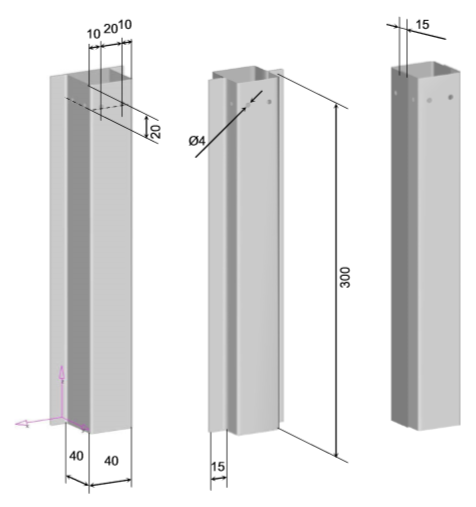
\includegraphics[angle=0,width=0.8\columnwidth]{crash_box}
\caption{General measures of the crash box model with the three different sections. Taken from \citet{Peroni2009}}
\label{fig:damage_evo2D}
\end{figure}

\citet{Scattina2011} tried square sections three different union layouts:
\begin{itemize}
\item Double hat section \citep{Lee2006, Yang2012, Yamashita2013}
\item Top hat \citep{Yamashita2013}
\item Bonding on square sides
\end{itemize}
\citet{Peroni2009} also tested two more union layouts, although they were discarded due to serious bond casting difficulties.

Comparison between cross-sections is possible as each possibility has the same box perimeter and the same bonding surface \citep{Peroni2009}.

\subsection{Triggering}

The trigger system consists on a series of holes placed at $\SI{20}{\mm}$ measured from the crushing end, with a diameter of $\SI{4}{\mm}$. They are meant to weaken the section in which they are applied in order to initiate collapse in that point. Collapse should start as a first wave in that cross-section if triggering has been correctly applied.

% Comment other triggers

\subsection{Impact conditions}  % Speed, etc

The tube was placed between two circular rigid plates, one next to the impact head and the rear one next to the opposite end. The impact plate had a initial separation of $\SI{1}{\mm}$ to avoid simulation problems.

The impact plate moved during the simulation at $\SI{10}{\m/\s}$ on a total distance equal to half of the total tube's length, resulting in a total analysis time of $\SI{0.015}{\s}$ long. Rotational \glspl{DOF} were fixed.

The rear plate had all \glspl{DOF} restrained. The reaction force that appeared on this point was used to measure \gls{Ea}, as explained later on (see \ref{sec:Ea}).

The last $\SI{5}{\mm}$ of the crash tube had all \glspl{DOF} fixed, except displacement on the impact direction in order to allow the reaction force measurement commented before. This way, numerical issues due to excesive \glspl{DOF} on the whole tube were prevented.

\subsubsection{Rivets}

\subsubsection{Stabilizing box}

After having faced strong difficulties to avoid \ref{sec:critical_sits}, four rigid plates on a rectangular section among the crash tube were added to the model as a stabilizing box. It had half of the length of the tube and moved toghether with the impact plate, so the crash tube would end confined between the plates on both ends and the stabilizing box by the end of the simulation.

% Numerical stabil justification
% Real sit justification

\subsection{Scripting}

Excepting some details added in the last phases of the development of the present study, the whole model has been scripted, making use of the Python interpreter integrated in Abaqus. This will allow model optimization in future phases of development. The script includes dimensional parameters, such as tube length or impact speed, and different cross sections (square and hexagonal), among other capabilities.

\section{Materials}

\subsection{Adhesive}
Loctite Hysol 9514 was the chosen adhesive for the bonding, for its shown interest by many other authors for structural bonding \citep{Sadowski2010, Scatina2011, SernaMoreno2015}, making it a priori a good candidate for the studied application.

\subsubsection{Density}
The adhesive's density was $\SI{14.6}{\tonne/\m^3}$ \citep{manufCatalog}, although some \ref{sec:mass_scaling} was applied for numerical issues (see the corresponding section). \citet{Scattina2011} pointed that results did not vary significantly, which was checked to be true.  % Not very happy with this

\subsubsection{Elastic behaviour}
\label{sec:elastic}
It was supposed to be isotropic linear elastic \citep{SernaMoreno2015} up to failure start. An uncoupled traction elastic behaviour \citep{Sadowski2010, Sadowski2011, Scattina2011, Sadowski2014} on \glspl{COH3D} was the best fit for modelling adhesives \citep{Abaqus613Manual}. Equation \ref{eq:traction} shows how this model works.

\begin{equation}
\label{eq:traction}
\begin{Bmatrix}
 t_n \\
 t_s \\
 t_t \\
\end{Bmatrix}
 =
\begin{bmatrix}
 E_{nn} & & \\
 & E_{ss} & \\
 & & E_{tt} \\
\end{bmatrix}
\begin{Bmatrix}
 \epsilon_n \\
 \epsilon_s \\
 \epsilon_t \\
\end{Bmatrix}
\end{equation}
% ######
% JACOBO: \caption sólo vale para figuras y tablas. A las ecuaciones no se les pone
% \caption{Uncoupled traction elastic constitutive equation. Taken from \citet{Abaqus613Manual}}

where $t_n$ is the nominal traction in the normal direction; $t_s$ and $t_t$ are the nominal traction in both shear directions; $E_{nn}$, $E_{ss}$ and $E_{tt}$ are the corresponding stiffnesses; and $\epsilon_n$, $\epsilon_s$ and $\epsilon_t$ are the corresponding nominal strains \citep{Abaqus613Manual}. $E_{ss}$ is considered equal to $E_{tt}$, and this value will be refered as $E_{T}$ onwards. In order to match this nomenclature, $E_{nn}$ will be refered as $E_{N}$.

This is an orthotropic model that only applies in one direction: the stack direction, as refered in \ref{sec:coh_elem}. The reduced adhesive layer thickness makes in-plane compression negligible. This situation also makes the coupling between components very difficult, so it's not considered.

\citet{Scattina2011} obtained adhesive stiffnesses through the inverse method, which are summarized in table \ref{tab:ads_params}. This same parameters were used in the present study.

\begin{table}
\begin{tabular}{llr}

 \toprule

 Parameter & Description & Value  \\

 \midrule

 $E_{N}$ & Stiffness in normal direction & $\SI{5e9}{\kN/\m^2}$ \\
 $E_{T}$ & Stiffness in an in-plane direction & $\SI{8e7}{\kN/\m^2}$ \\

 \bottomrule

\end{tabular}
\caption{Loctite Hysol 9514 parameters. Taken from \citet{Scattina2011}}
\label{tab:ads_params}
\end{table}

The value of $E_{N}$ can be calculated by dividing the elastic modulus, $E$, by the adhesive layer thickness. This elastic modulus is calculated using bulk modulus, $K$, provided by \citet{manufCatalog} and a Poisson's modulus, $\nu$, of $\num{0.295}$ \citep{JDiaz}.

\subsubsection{Damage model}
% Check other authors here
\citet{Wu2013} showed the two possible failure mechanisms an adhesive union may show: 
\begin{itemize}
\item Adhesive failure, refered to the contact between different materials, implies the separation of the adhesive from the adherend.
\item Cohesive failure \citep{Vaidya2006}, refered to the bulk material, means that one piece of adhesive gets teared apart from another, breaking the continuum.
\end{itemize}

Contact failure modelling resulted in some simulation problems. Elements separating alternativelly from each adherend appeared toghether with elements inbetween in good state. Instead of getting stiffness degradation in the whole adhesive, each of those healthy elements was subjected to the load its neighbours weren't handling, and thus failing significantly reducing adhesive's overall resistance, apart from other numerical issues.

This situation was overcome by including only failure definitions in the bulk material, obviating the contact failure \citep{Greve2007, Loureiro2010, Sadowski2010, Sadowski2011, Scattina2011, Sadowski2014, SernaMoreno2015}, although the modelled cohesive damage includes the effect of both adhesive and cohesive resistance.

The \gls{quads}, which can be seen in equation \ref{eq:quads}, is a widelly used damage initiation criterion \citep{Greve2007, Loureiro2010, Sadowski2010, Sadowski2011, Scattina2011, Sadowski2014, SernaMoreno2015}.

\begin{equation}
\left(\frac{\left<\sigma_{n}\right>}{\sigma_{n}^{0}}\right)^{2} + \left(\frac{\tau_{II}}{\tau_{II}^{0}}\right)^{2} + \left(\frac{\tau_{III}}{\tau_{III}^{0}}\right)^{2} = 1
\label{eq:quads}
\end{equation}
% \caption{Quadratic nominal stress criterion equation}

where $\sigma_{n}^{0}$, $\tau_{II}^{0}$ and $\tau_{III}^{0}$ represent the pure mode loading threshold stresses for each direction. The out-of-plane value, $\sigma_{n}^{0}$, was set to $\SI{42.5}{\MPa}$ \citep{Scattina2011}, which corresponds to the peeling failure stress for steel. Note that Macaulay brackets indicate that compression is not considered in failure initiation. Both in-plane values, $\tau_{II}^{0}$ and $\tau_{III}^{0}$, were set to $\SI{130}{\MPa}$ \citep{Scattina2011}. % ref to catalog?

As long as the condition is not satisfied, the adhesive layer behaves elastically. Once the condition gets satisfied, damage starts and a degradation in stiffness can be appreciated following the especified damage evolution model, being thus a case of \gls{LEFM}, as the traction behaviour is also linear.

\gls{XFEM}-based \gls{LEFM} require a pre-existing crack in the model or some nucleation formulation that governs its propagation \citep{Abaqus613Manual}. As the crack's initial localization and direction is not previously known, the \gls{VCCT} criterion is used. This technique can be applied in brittle crack formation, which is the case, as no plastification happens before damage or failure.

For this particular case, the \gls{VCCT} formulation was set as a fracture energy power law \citep{Loureiro2010, Sadowski2010, Sadowski2011, Sadowski2014, SernaMoreno2015}, as the given by equation \ref{eq:fracture_energy}.

\begin{equation}
\left(\frac{G_{I}}{G_{Ic}}\right)^{\alpha}+\left(\frac{G_{II}}{G_{IIc}}\right)^{\alpha}+\left(\frac{G_{III}}{G_{IIIc}}\right)^{\alpha}=1
\label{eq:fracture_energy}
\end{equation}
% \caption{Fracture energy power law model equation}

where $G_{Ic}$ corresponds to the critical fracture energy required to cause failure in mode I (out-of-plane direction), and being $G_{IIc}$ and $G_{IIIc}$ the values for mode II and III, respectively, which correspond to both in-plane directions. The critical fracture energy for the Loctite Hysol 9514 in the normal direction is $\SI{2028}{\J/\m^2}$ \citep{Scattina2011}. It was considered that the adhesive had no preferential directions for tangential failure, meaning $G_{IIc}$ was equal to $G_{IIIC}$, and being the fracture energy equal to $\SI{11853}{\J/\m^2}$ \citep{Scattina2011}. The exponent $\alpha$ was considered equal to $\num{2}$ \citep{Loureiro2010, Sadowski2010, Sadowski2011, Sadowski2014, SernaMoreno2015}.

Once damage has started, according to this model, fracture energy is released as damage progresses reducing material stiffness. If unloaded, the material would behave elastically again with degraded properties until damage criterion is accomplished again. Figure \ref{fig:damage_evo2D} illustrates this behaviour for a simplified 2D case.

\begin{figure}
\centering
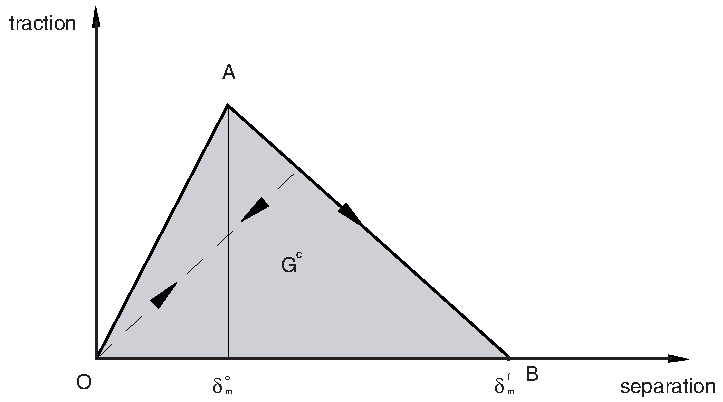
\includegraphics[angle=0,width=0.8\columnwidth]{damage_evolution_manual}
\label{fig:damage_evo2D}
\end{figure}
% \caption{Damage evolution representation for a 2D case. Taken from \citep{Abaqus613Manual}}

Figure \ref{fig:damage} represents the whole damage model, including damage initiation and the fracture energy, which corresponds to the area beneath the curve.

\begin{figure}
\centering
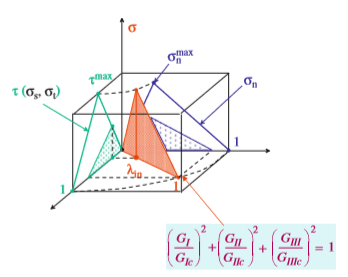
\includegraphics[angle=0,width=0.8\columnwidth]{QUADS}
\caption{Damage model representation. Taken from \citep{Sadowski2010}}
\label{fig:damage}
\end{figure}

\begin{table}
\begin{tabular}{llr}

 \toprule

 Parameter & Description & Value  \\

 \midrule

 $G_{Ic}$ & Energy release rate for mode I & $\SI{2028}{\J/\m^2}$ \\
 $G_{IIc}$ & Energy release rate for mode II & $\SI{11853}{\J/\m^2}$ \\
 $\sigma_{n}^{0}$ & Peak traction in normal direction & $\SI{130}{\MPa}$ \\
 $\tau_{II}^{0}$ & Peak traction in tangential direction & $\SI{42.5}{\MPa}$ \\

 \bottomrule

\end{tabular}
\caption{Summary of Loctite Hysol 9514 damage parameters. Taken from \citet{Scattina2011}}
\label{tab:ads_dmg_params}
\end{table}

\subsubsection{Comparison of input with \citet{ManufCatalog} data}

\subsubsection{\Gls{SLJ}}

\subsection{Adherend}

\section{Computation}

\subsection{Software}

\subsection{Numerical issues}
% Include computational time

\subsubsection{Mesh}

The use of \glspl{COH3D} allowed to make the adhesive's mesh much coarser due to their aspect ratios requirements. These elements were seeded with a size of $\SI{2.0}{\mm}$, and had only one element in the $\SI{0.3}{\mm}$ layer thickness. Other tried element types had problems if seeds were bigger than about $\SI{0.5}{\mm}$, and were completelly unfeasible with seeds bigger than $\SI{1.0}{\mm}$ approximatedly.

% Mesh divisions for structure
% Tie (include image)
% Total recount of elements (by part?)

\subsubsection{The cohesive element}
\label{sec:coh_elem}
\citep{Alfano2001, Greve2007, Carlberger2007, Alvarez2014, May2014}

As \glspl{COH3D} were especifically formulated for adhesive modelling, among other uses, they have been widelly used to model this material, in Abaqus \citep{Sadowski2010, Sadowski2011, Sadowski2014, Alvarez2014} and in other software packages \citep{Sato2000, Carlberger2007, Loureiro2010, Scattina2011, Ghasemnejad2013}, although this is not the only existing formulation \citep{Sato2000, Greve2007, Liao2011, Yang2012}. Certain stress distributions cannot be properlly modelled, but these have no interest or negligible effects. In-plane compression is an example that illustrates this situation.

\Glspl{COH3D} geometrically require:
\begin{itemize}
\item There can only be a single layer of elements.
\item Element's shape must be plate-like: height smaller than the other dimensions, but not negligible.
\item A stack direction, usually based on the first point.
\end{itemize}
As the adhesive layer is very thin, it matches this geometrical requirements, making these elements suitable for this application. These needed aspect ratios allow a coarser mesh with good results.

The \gls{VCCT} strongly penalizes the minimum stable time increment \citep{Abaqus613Manual}, reducing it even to the order of $\SI{1.5e-9}{\s}$, much more unfavorable if compared to other damage models tried during the development of this study, which made it about $\SI{2e-7}{\s}$.

\subsubsection{Mass scaling}
\label{sec:mass_scaling}
Following \citet{Scattina2011}, mass scaling was applied to the adhesive's density in order to improve numerical performance. Increasing it one order of magnitude results on a stable time increment up to 30 times bigger. Increasing it two orders of magnitude results in very similar improvements, a bit worse perhaps.

Quasi-static models were carried out scaling adhesive's density, as the total simulation time made it necesary in order to obtain results at a far more reasonable computational cost. A factor of 40 was used, resulting in stable time increments almost two orders of magnitude bigger than the original ones.

